\documentclass{beamer}
\graphicspath{{images/}}

\title{Intro to Git}
\date{}

\begin{document}

\frame{\titlepage}

\begin{frame}
	\frametitle{Plan}
	\begin{itemize}
		\item{Intro to Version Control}
		\item{Getting Started}
		\item{Git Basics}
		\item{Branches in Git}
		\item{Git Reset in Detail}
	\end{itemize}
\end{frame}

% Section 1: Into to Version Control

\begin{frame}
	\frametitle{Intro to Version Control}
	\begin{itemize}
		\item{System that records changes to a file or set of files over time (VCS)}
		\item{Can recall specific versions at a later time}
		\item{Can revert individual files or even the entire project to a previous state}
		\item{Can compare changes in files over time}
		\item{Can see who modified something and when}
		\item{Does the very efficiently}
		\item{Set of all versions of all files called a repository}
	\end{itemize}
\end{frame}

\begin{frame}
	\frametitle{Local VCS}
	\begin{itemize}
		\item{Simple database containing all changes to file under version control}
	\end{itemize}
	\begin{figure}
		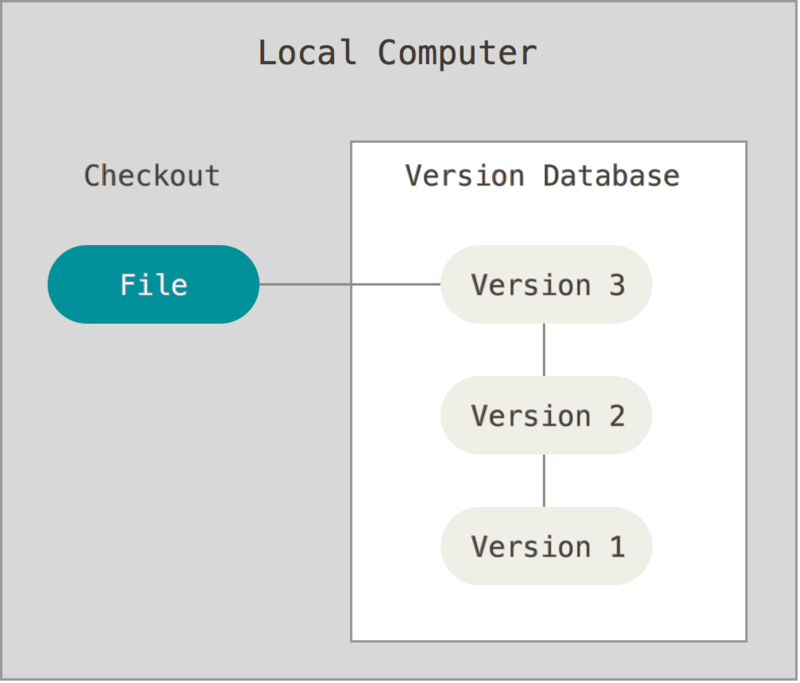
\includegraphics[scale=0.25]{Local_VCS-0.png}
	\end{figure}
\end{frame}

\begin{frame}
	\frametitle{Centralised VCS}
	\begin{itemize}
		\item{Used to collaborate with other developers}
		\item{Single server contains all the versioned files}
		\item{Clients check out snapshots from the server}
	\end{itemize}
	\begin{figure}
		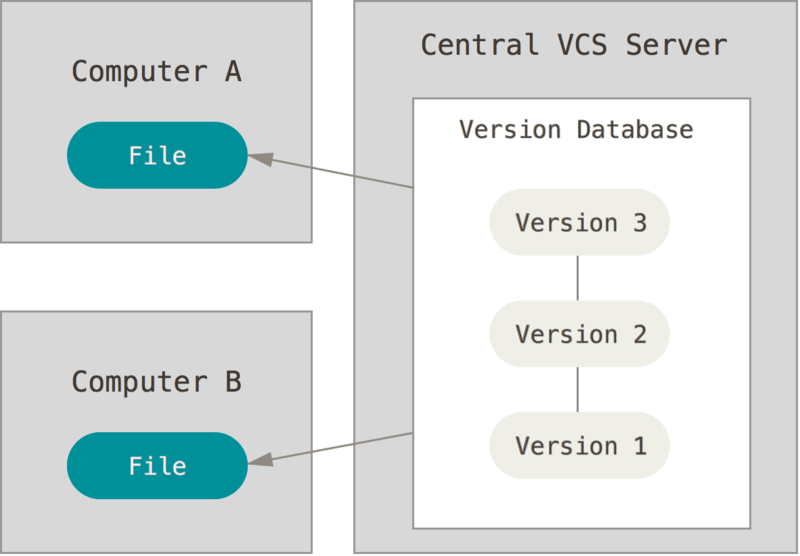
\includegraphics[scale=0.25]{Centralised_VCS-0.png}
	\end{figure}
\end{frame}

\begin{frame}
	\frametitle{Distributed VCS}
	\begin{itemize}
		\item{Each client fully mirrors the the repository}
		\item{Allows direct collaboration between developers}
	\end{itemize}
	\begin{figure}
		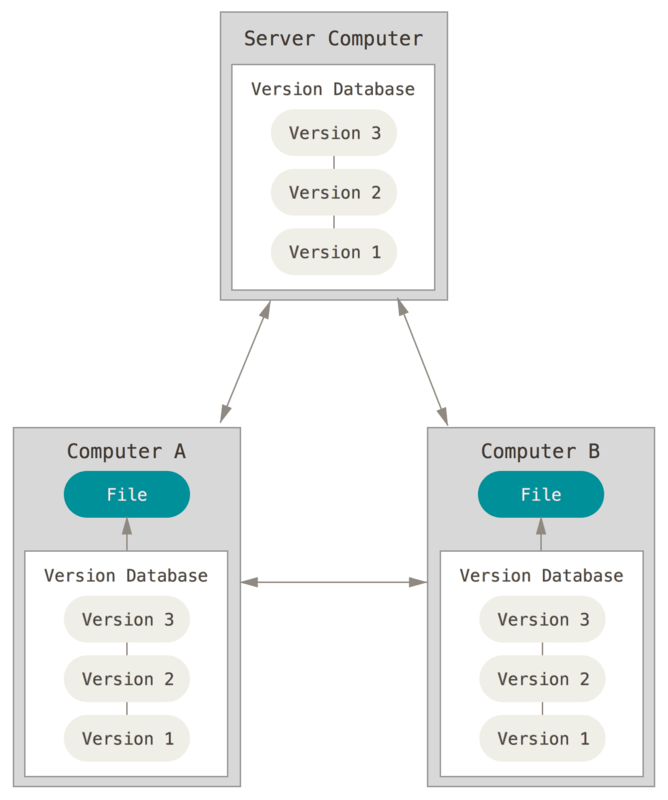
\includegraphics[scale=0.25]{Distributed_VCS-0.png}
	\end{figure}
\end{frame}

% Section 2: Getting Started

\begin{frame}
	\frametitle{A Short History of Git}
	\begin{itemize}
		\item{Created by Linus Torvalds in 2005 for Linux kernel development}
		\item{The goals for Git were:}
		\begin{itemize}
			\item{Speed}
			\item{Simple design}
			\item{Able to handle large projects}
			\item{Fully distributed}
			\item{Very good support for non-linear development}
		\end{itemize}
	\end{itemize}
\end{frame}

\begin{frame}
	\frametitle{Differences}
	\begin{itemize}
		\item{Store initial file version and each change over time}
	\end{itemize}
	\begin{figure}
		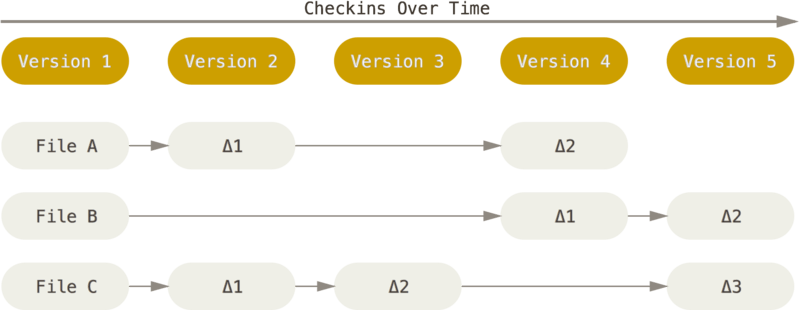
\includegraphics[scale=0.25]{Differences-0.png}
	\end{figure}
\end{frame}

\begin{frame}
	\frametitle{Snapshots}
	\begin{itemize}
		\item{Every time you commit (save) the project state, a new snapshot of is made}
		\item{A snapshot is a "picture" of all the files in the repo}
		\item{Files that haven't changed aren't saved for efficiency}
	\end{itemize}
	\begin{figure}
		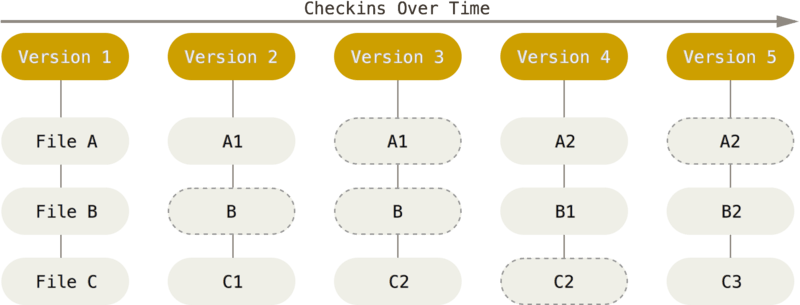
\includegraphics[scale=0.25]{Snapshots-0.png}
	\end{figure}
\end{frame}

\begin{frame}
	\frametitle{Almost everything in Git is local}
	\begin{itemize}
		\item{Most operations in Git only affect your local copy of the repo}
		\item{Very rarely need to go onto the network}
		\item{No network latency}
		\item{Can work offline}
	\end{itemize}
	\begin{figure}
		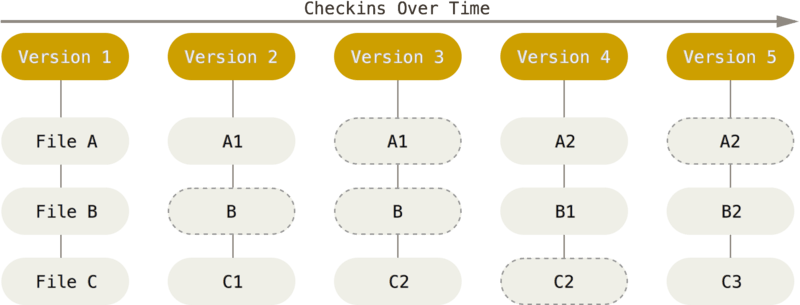
\includegraphics[scale=0.25]{Snapshots-0.png}
	\end{figure}
\end{frame}

\begin{frame}
	\frametitle{Git has built-in integrity checking}
	\begin{itemize}
		\item{Everything stored in Git is check-summed}
		\item{Changing something changes the checksum and the history}
		\item{Git is able to detect any file corruption or modification}
		\item{24b9da6552252987aa493b52f8696cd6d3b00373}
		\item{SHA-1 hash (40-char hex string)}
	\end{itemize}
\end{frame}

\begin{frame}
	\frametitle{The Three States}
	\begin{itemize}
		\item{One of the most important things in Git}
		\item{Files in your repository exist in one of three states}
		\item{Committed: Safely stored in your local database}
		\item{Modified: Changed a file but not committed it yet}
		\item{Staged: Marked a modified file to go in the next commit snapshot}
	\end{itemize}
	\begin{figure}
		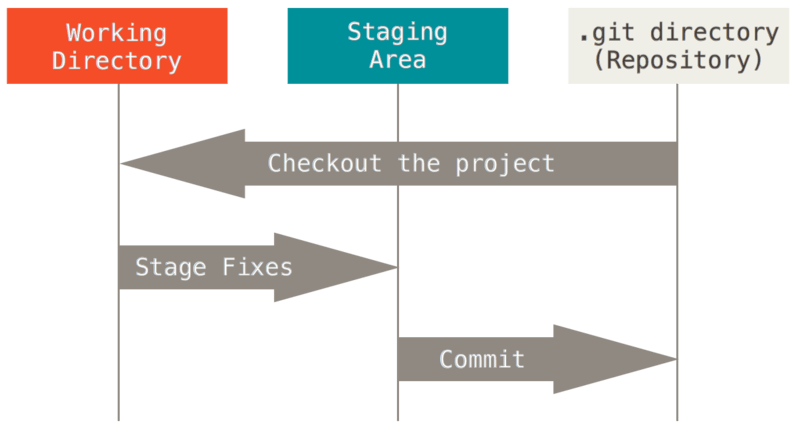
\includegraphics[scale=0.25]{The_Three_States-0.png}
	\end{figure}
\end{frame}

\begin{frame}
	\frametitle{The Three States}
	\begin{itemize}
		\item{The .git directory is where Git stores the snapshots}
		\item{The working tree is a single snapshot of the repository}
		\item{Uncompressing a snapshot from .git is called "checking out"}
		\item{The staging area stores information about what goes into the next commit}
	\end{itemize}
\end{frame}

\begin{frame}
	\frametitle{Development Cycle}
	\begin{itemize}
		\item{1. Modify files in working tree}
		\item{2. Stage some of the modified files}
		\item{3. Do a commit, saving the contents of the staging area into a new snapshot}
	\end{itemize}
\end{frame}

\begin{frame}
	\frametitle{Installing Git}
	\begin{itemize}
		\item{Available on Linux, Windows, Mac}
		\item{Package managers or from source at https://github.com/git/git/releases}
	\end{itemize}
\end{frame}

\begin{frame}
	\frametitle{First Time Configuration}
	\begin{itemize}
		\item{Configuration in git is done with the \textbf{git config} command}
		\item{This command allows you to get and set configuration variables}
		\item{These variables can be stored in three different places}
		\item{/etc/gitconfig file: System-wide values, use --system switch}
		\item{\textasciitilde{}/.gitconfig or \textasciitilde{}/.config/git/config file: This user only, use --global switch}
		\item{.git/config file: This repository only, no switch required}
	\end{itemize}
\end{frame}

\begin{frame}
	\frametitle{First Time Configuration}
	\begin{itemize}
		\item{\textbf{git config \texttt{-{}-}global user.name "Sam Caulfield"}}
		\item{\textbf{git config user.email "sam.caulfield@movidius.com"}}
		\item{\textbf{git config \texttt{-{}-}system core.editor "vim"}}
		\item{Precedence: Per Repository \textgreater{} Per User \textgreater{} System}
		\item{Show configuration settings with \textbf{git config \texttt{-{}-}list}}
		\item{Show just one configuration option with \textbf{git config user.name}}
	\end{itemize}
\end{frame}

\begin{frame}
	\frametitle{Getting help}
	\begin{itemize}
		\item{\textbf{git help \textless{}verb\textgreater{}}}
		\item{\textbf{git \textless{}verb\textgreater{} \texttt{-{}-}help}}
		\item{\textbf{man git-\textless{}verb\textgreater{}}}
		\item{https://git-scm.com/book/en/v2/}
	\end{itemize}
\end{frame}

% Section 3: Git Basics

\begin{frame}
	\frametitle{Getting a Git Repository}
	\begin{itemize}
		\item{Two main ways: create one or copy one}
		\item{To create one: \textbf{git init} or \textbf{git init MyRepo}}
		\item{To copy one: \textbf{git clone https://github.com/libgit2/libgit2}}
	\end{itemize}
\end{frame}

\begin{frame}
	\frametitle{Recording Changes to the Repository}
	\begin{itemize}
		\item{Need to make changes and commit snapshots}
		\item{Files in the working directory are either tracked or untracked}
		\item{Tracked: Present in the previous snapshot}
		\item{Untracked: Not present in the previous snapshot or in the staging area}
		\item{Tracked files can be unmodified, modified, or staged}
	\end{itemize}
	\begin{figure}
		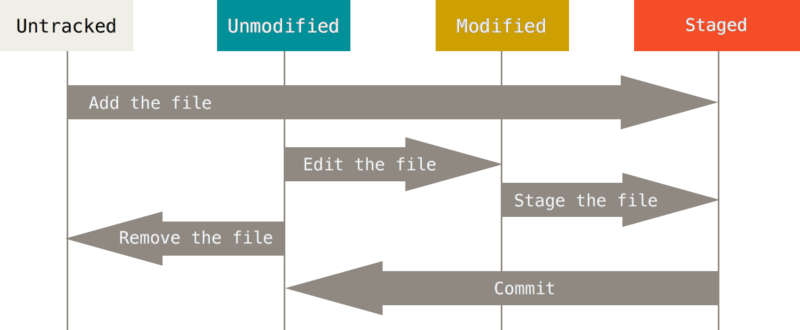
\includegraphics[scale=0.37]{Recording_Changes_to_the_Repository-0.png}
	\end{figure}
\end{frame}

\begin{frame}
	\frametitle{Checking the Status of Files}
	\begin{itemize}
		\item{Done with the \textbf{git status} command}
	\end{itemize}
	\begin{figure}
		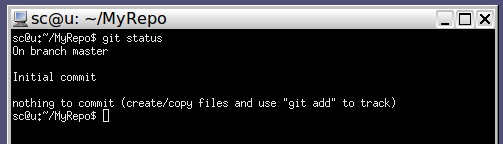
\includegraphics[scale=0.50]{Checking_the_Status_of_Files-0.png}
	\end{figure}
	\begin{figure}
		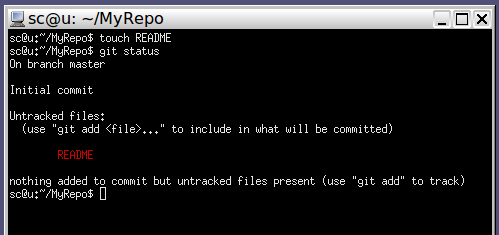
\includegraphics[scale=0.50]{Checking_the_Status_of_Files-1.png}
	\end{figure}
\end{frame}

\begin{frame}
	\frametitle{Tracking New Files}
	\begin{itemize}
		\item{Done with the \textbf{git add} command}
	\end{itemize}
	\begin{figure}
		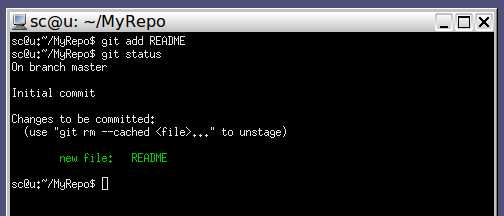
\includegraphics[scale=0.50]{Tracking_New_Files-0.png}
	\end{figure}
\end{frame}

\begin{frame}
	\frametitle{Staging Modified Files}
	\begin{figure}
		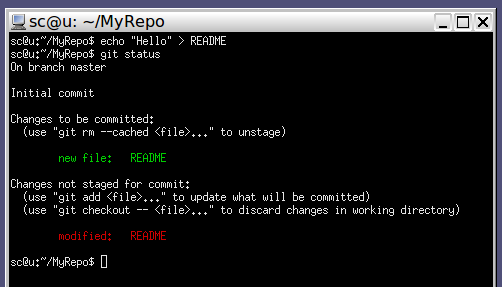
\includegraphics[scale=0.60]{Staging_Modified_Files-0.png}
	\end{figure}
\end{frame}

\begin{frame}
	\frametitle{Staging Modified Files}
	\begin{itemize}
		\item{Done with the \textbf{git add} command}
		\item{\textbf{git add \texttt{-{}-}patch} can be used to stage parts of files}
	\end{itemize}
	\begin{figure}
		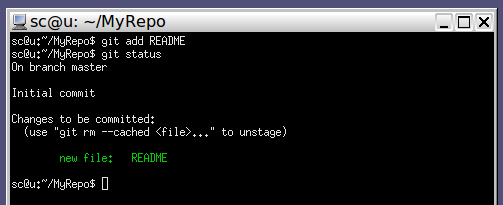
\includegraphics[scale=0.60]{Staging_Modified_Files-1.png}
	\end{figure}
\end{frame}

\begin{frame}
	\frametitle{Short Status}
	\begin{itemize}
		\item{\textbf{git status -s} provides a less verbose status report}
		\item{Untracked files have a ?? next to them}
		\item{New files that have been added to the staging area have an A}
		\item{Modified files have an M, etc.}
		\item{Left column: index, right column: working directory}
	\end{itemize}
	\begin{figure}
		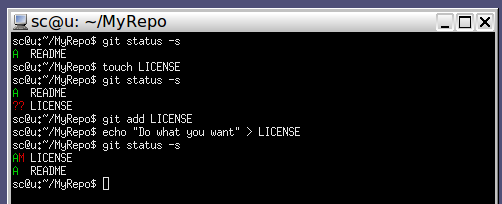
\includegraphics[scale=0.62]{Short_Status-0.png}
	\end{figure}
\end{frame}

\begin{frame}
	\frametitle{Ignoring Files}
	\begin{itemize}
		\item{The working directory can easily become full of files you don't want to version}
		\item{.o, .swp, .log, etc.}
		\item{They can clog up the output of \textbf{git status}}
		\item{List unwanted file types in a .gitignore file in the repository}
		\item{\textbf{echo *.o \textgreater{} .gitignore}}
		\item{Can perform simple pattern matching: doc/**/*.pdf}
	\end{itemize}
\end{frame}

\begin{frame}
	\frametitle{Viewing Staged and Unstaged Changes}
	\begin{itemize}
		\item{What have I changed but not staged?}
		\item{What have I staged that I am about to commit?}
		\item{Use the \textbf{git diff} command}
		\item{This shows what's changed in the working directory that isn't staged}
	\end{itemize}
	\begin{figure}
		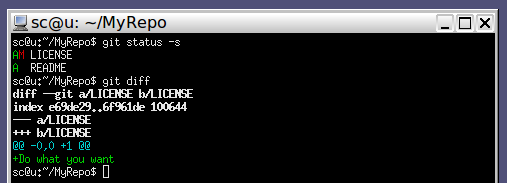
\includegraphics[scale=0.62]{Viewing_Staged_and_Unstaged_Changes-0.png}
	\end{figure}
\end{frame}

\begin{frame}
	\frametitle{Viewing Staged and Unstaged Changes}
	\begin{itemize}
		\item{To view what's new in the staging area use \textbf{git diff --staged}}
	\end{itemize}
	\begin{figure}
		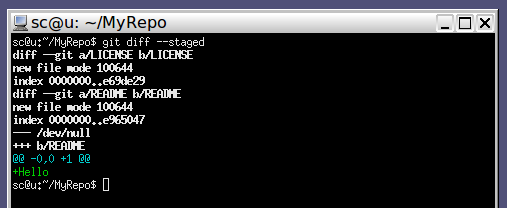
\includegraphics[scale=0.62]{Viewing_Staged_and_Unstaged_Changes-1.png}
	\end{figure}
\end{frame}

\begin{frame}
	\frametitle{Committing Your Changes}
	\begin{itemize}
		\item{Committing creates a new snapshot in the project history}
		\item{The snapshot is the previous snapshot + the staging area changes}
		\item{Anything left in the working directory and not in the staging area isn't included}
		\item{Use the \textbf{git commit} command}
	\end{itemize}
	\begin{figure}
		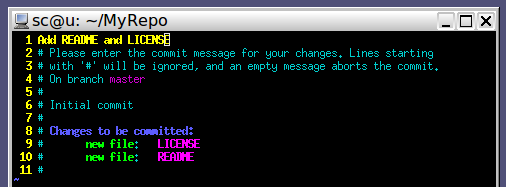
\includegraphics[scale=0.62]{Committing_Your_Changes-0.png}
	\end{figure}
\end{frame}

\begin{frame}
	\frametitle{Committing Your Changes}
	\begin{itemize}
		\item{Saving and closing the editor confirms the commit}
		\item{Alternatively, you can use \textbf{git commit -m "Add README and LICENSE"}}
		\item{Can skip staging with \textbf{git commit -a}}
	\end{itemize}
	\begin{figure}
		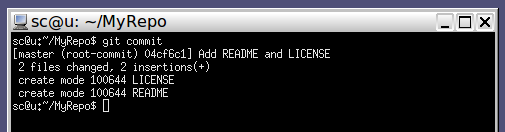
\includegraphics[scale=0.62]{Committing_Your_Changes-1.png}
	\end{figure}
\end{frame}

\begin{frame}
	\frametitle{Removing Files from the Repository}
	\begin{itemize}
		\item{Use the \textbf{git rm} command}
	\end{itemize}
	\begin{figure}
		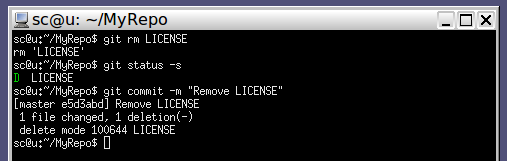
\includegraphics[scale=0.62]{Removing_Files_from_the_Repository-0.png}
	\end{figure}
	\begin{itemize}
		\item{Similarly, \textbf{git mv} can be used to move files}
	\end{itemize}
\end{frame}

\end{document}
